\begin{figure*}[t]
  \begin{minipage}[t]{0.496\linewidth}
    \centering
    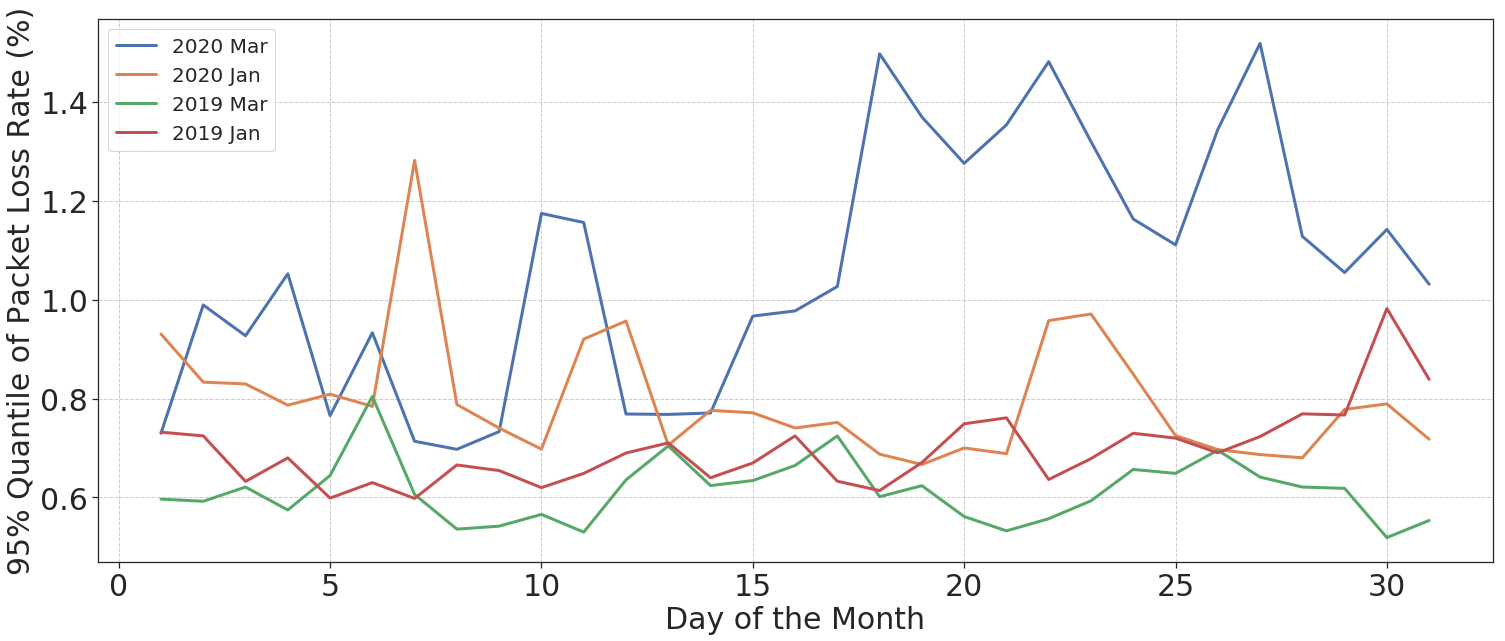
\includegraphics[width=0.98\linewidth]{figs/packet_loss_per_day.png}
    \caption{Graph comparing the 95\% quantile packet loss per day for the months January, March 2019 and January, March 2020.}
    \label{fig:packetlossperday}
  \end{minipage}
  \begin{minipage}[t]{0.496\linewidth}
    \centering
    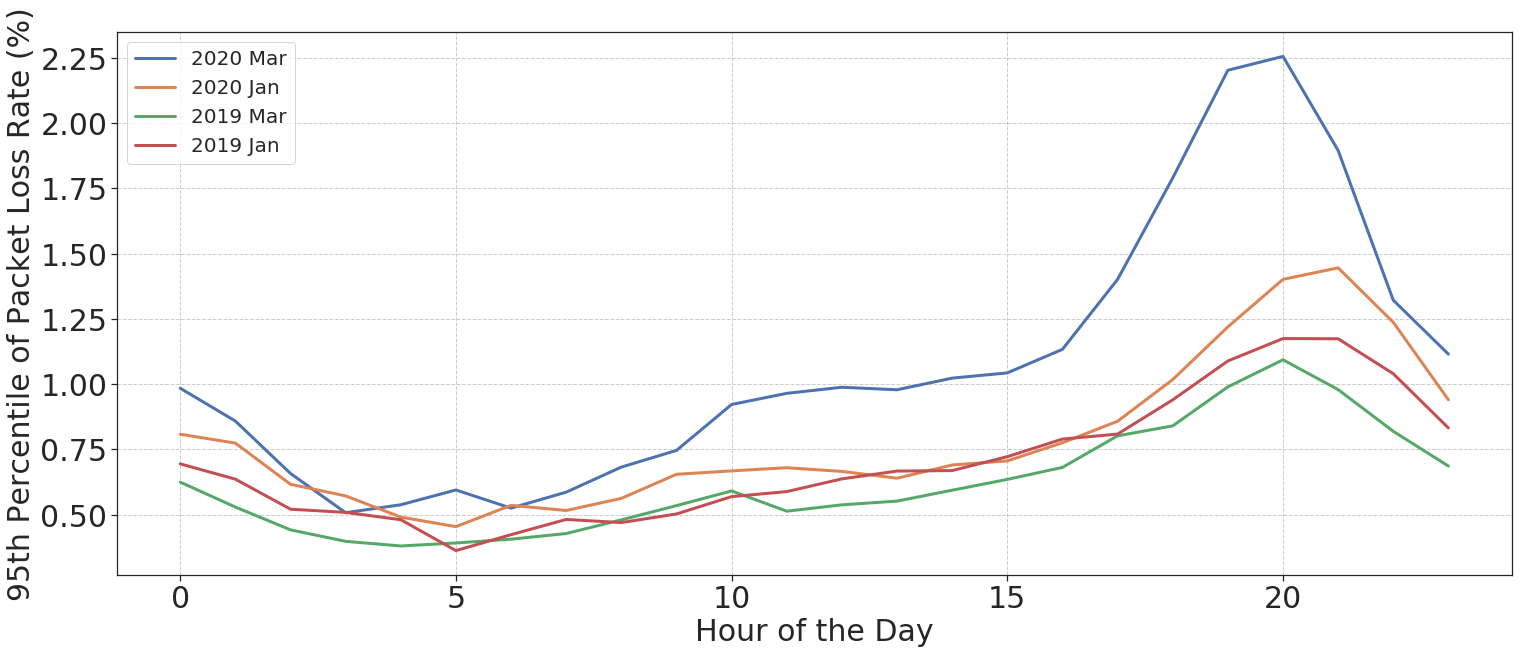
\includegraphics[width=0.98\linewidth]{figs/packet_loss_per_hour.png}
    \caption{Graph comparing the 95\% quantile packet loss per hour for the months January, March 2019 and January, March 2020.}
    \label{fig:packetlossperhour}
  \end{minipage}
\end{figure*}

\section{Packet Loss Analysis}\label{sec:packet-loss-analysis}

Apart from studying data usage and connection speed patterns, we can also examine the effects of COVID-19 restrictions on packet loss. With increasing fixed broadband internet usage during the lockdown period, network congestion is also likely to increase. Increasing network congestion will manifest itself in increasing packet loss.

Each test unit performs a \gls{UDP} latency measurement periodically throughout the day. During the measurement, the test unit sends a series of \gls{UDP} datagrams to a pre-defined set of servers. Parameters such as minimum, maximum, and average round  trip time are recorded, as well as the number of lost \gls{UDP} packets. The \gls{UDP} test is only performed when there is no user activity on the connection. Thus, the results are primarily influenced by the performance of the fixed broadband connection rather than local user traffic.

We use number the total number of sent and lost \gls{UDP} datagrams to calculate packet loss rate. To quantify the packet loss rate for one test unit, we define the metric as:

\begin{equation}
    Packet \ Loss\, \% = \frac{\#Failure }{\#Failure + \#Success} \times 100
\end{equation}

Previous studies~\cite{kovacs} suggested that the majority of the \gls{US} did not experience any degradation of network performance. We thus focus on the subset of the users that did experience network degradation and study packet loss at the 95\% quantile, i.e., users at the higher end of the packet loss spectrum.

\subsection{Daily Packet Loss}

\cref{fig:packetlossperday} shows the 95\% quantile of daily packet loss over January and March 2019 and 2020. We see a significant increase in packet loss starting from mid-March 2020. Mid-March is the period when some \gls{US} states began imposing statewide lockdown orders. In this time period, the packet loss rate grows by 40--50\% compared to early March 2020, which is before the pandemic. Towards the end of March 2020, packet loss rate is 80\% higher than that before the pandemic, implying that some network congestion might occur.

Since we do not observe similar trends in 2019, this suggests that this increase is not due to noise and might be instead due to the additional traffic generated by activities such as work from home, distance learning, and video conferencing. This increase also coincides with the increase in downloaded data we observed in metro areas in \cref{fig:downloadmetro_rural}.

%Note, however, that by the end of March the loss rate again starts to decrease. We speculate that this might be due to the rapid response of network and service operators who rapidly began adding capacity to meet the increasing need \cite{liu2020characterizing}.

\subsection{Hourly Packet Loss}

In this section, we examine the influence of the hour of the day on packet loss. \cref{fig:packetlossperhour} depicts the 95\% quantile of packet loss over the course of a day in January, March 2019 and 2020. We found the packet loss ratio changing over the course of the day, with the maximum around 20:00. This is consistent with data upload and download patterns discussed earlier.

In March 2020, the packet loss rate increased steeply during daytime from 7:00 to 22:00, potentially due to the users' growing online activities like remote learning, work from home, etc. However, this change was more evident during the evening. For example, we saw an around 59\% growth from 18:00 to 22:00 when comparing March to January 2020. This time period lies outside of traditional working hours, suggesting that packet loss is more positively related to the increased traffic due to recreational activities rather than remote working or distance learning.

Our results are consistent with Candela et al.~\cite{Candela2020latency}, as they found the increase of packet loss might be affected by factors like the type of server, \gls{IP} version, and the time of the day.

%\subsection{95\% Hourly Packet Loss}
%Besides, we notice the same slight increase of capacity loss through the hourly packet loss data.
